\documentclass{beamer}

\usetheme{default}
\usepackage{helvet}
\usepackage[utf8]{inputenc}
\PassOptionsToPackage{hyphens}{url}\usepackage{hyperref,xspace,multicol}
\usepackage[absolute,overlay]{textpos}
\usepackage{tikz}
\usetikzlibrary{arrows,shapes,trees,shadows,positioning}
\usepackage{tree}
\usepackage{fancyvrb}           % for \Verb

% Remember the position of every picture.
\tikzstyle{every picture}+=[remember picture]

\tikzset{onslide/.code args={<#1>#2}{%
  \only<#1>{\pgfkeysalso{#2}} % \pgfkeysalso doesn't change the path
}}

% Colors.
\definecolor{guixred1}{RGB}{226,0,38}  % red P
\definecolor{guixorange1}{RGB}{243,154,38}  % guixorange P
\definecolor{guixyellow}{RGB}{254,205,27}  % guixyellow P
\definecolor{guixred2}{RGB}{230,68,57}  % red S
\definecolor{guixorange2}{RGB}{236,117,40}  % guixorange S
\definecolor{guixtaupe}{RGB}{134,113,127} % guixtaupe S
\definecolor{guixgrey}{RGB}{91,94,111} % guixgrey S
\definecolor{guixblue1}{RGB}{38,109,131} % guixblue S
\definecolor{guixblue2}{RGB}{28,70,114} % guixblue S
\definecolor{guixgreen1}{RGB}{133,146,66} % guixgreen S
\definecolor{guixgreen2}{RGB}{157,193,7} % guixgreen S

% White-on-black color theme.
\setbeamercolor{structure}{fg=guixorange1,bg=black}
\setbeamercolor{title}{fg=white,bg=black}
\setbeamercolor{date}{fg=guixorange1,bg=black}
\setbeamercolor{frametitle}{fg=white,bg=black}
\setbeamercolor{titlelike}{fg=white,bg=black}
\setbeamercolor{normal text}{fg=white,bg=black}
\setbeamercolor{alerted text}{fg=guixyellow,bg=black}
\setbeamercolor{section in toc}{fg=white,bg=black}
\setbeamercolor{section in toc shaded}{fg=white,bg=black}
\setbeamercolor{subsection in toc}{fg=guixorange1,bg=black}
\setbeamercolor{subsection in toc shaded}{fg=white,bg=black}
\setbeamercolor{subsubsection in toc}{fg=guixorange1,bg=black}
\setbeamercolor{subsubsection in toc shaded}{fg=white,bg=black}
\setbeamercolor{frametitle in toc}{fg=white,bg=black}
\setbeamercolor{local structure}{fg=guixorange1,bg=black}

% Commands from
% <https://svn.nixos.org/repos/varia/trunk/presentations/ghm-2009/doc.ltx>.
\newcommand{\code}[1]{{\tt #1}}
\newcommand{\symlink}{
  \pgfsetendarrow{\pgfarrowtriangle{4pt}}
  \pgfsetlinewidth{1pt}
  \pgfsetdash{{0.05cm}{0.05cm}}{0cm}
  \color{blue}
}


\title{We're building the GNU system!}

\author{Ludovic Courtès\\\texttt{ludo@gnu.org}}
\date{\small{GNU Hackers Meeting\\15 August 2014, München}}

\setbeamertemplate{navigation symbols}{} % remove the navigation bar

\AtBeginSection[]{
  \begin{frame}
    \frametitle{}
    \tableofcontents[currentsection, hideothersections]
  \end{frame} 
}


\AtBeginSubsection[]{
  \begin{frame}
  \frametitle{}
  \tableofcontents[currentsection, currentsubsection]
  \end{frame}
}

\begin{document}

\maketitle

\begin{frame}{Howdy!}
  \center{\includegraphics[width=0.7\textwidth]{images/guile-banner-white}}
  \\[0.8em]
  \uncover<2->{\center{
\includegraphics[width=0.4\textwidth]{images/nixos-white}}}
  \\

  \begin{textblock}{15}(0, 6)
    \tikz \node<3->[overlay, fill=black, opacity=.8, text height=5cm,
       text centered, text opacity=1, inner sep=10mm] at (0.5, -0.5) {
      \includegraphics[width=0.55\textwidth]{images/guix-logo-white}};
  \end{textblock}
\end{frame}

\begin{frame}[plain]
  \Huge{the ``\textbf{GNU system}'', \\
aka. ``a GNU distribution''}

  \vspace{0.5cm}
  \large{
    \begin{itemize}
      \item<2-> protect \& enhance \alert{computing freedom}
      \item<2-> improve \alert{integration} of GNU software, consistency
      \item<2-> improve \alert{workflow} among GNU hackers \& users
    \end{itemize}}
\end{frame}

\begin{frame}[plain]
  \begin{centering}
    \LARGE{Dependable.  Hackable.  Liberating.}
  \end{centering}
\end{frame}



%%%%%%%%%%%%%%%%%%%%%%%%%%%%%%%%%%%%%%%%%%%%%%%%%%%%%%%%%%%%%%%%%%%%%%%%%%%%%%%%
\begin{frame}[plain]
  \begin{centering}
    \Huge{\textbf{Dependable.}}
  \end{centering}
\end{frame}


\begin{frame}[fragile]
  \frametitle{per-user, transactional package installation etc.}

  \begin{semiverbatim}
alice@foo\$ \alert<1>{guix package --install=gcc}
\uncover<1->{alice@foo\$ \alert{guix gc --references `which gcc`}
/gnu/store/...-glibc-2.19
/gnu/store/...-gcc-4.9.1
...}

\uncover<1->{bob@foo\$ \alert{guix package --install=gcc-4.7.3}}
\uncover<1->{bob@foo\$ \alert{guix gc --references `which gcc`}
/gnu/store/...-glibc-2.17
/gnu/store/...-gcc-4.7.3
...}
  \end{semiverbatim}

  \begin{tikzpicture}[overlay]
    \node[rounded corners=4, text centered,
          fill=guixorange1, text width=3cm,
          inner sep=3mm, rotate=5, opacity=.75, text opacity=1,
          drop shadow={opacity=0.5}] at (5, 4) {
            \textbf{\large{demo!}}
          };
  \end{tikzpicture}
\end{frame}

\begin{frame}[fragile]
  \frametitle{transparent binary/source deployment}
  \begin{overlayarea}{\textwidth}{6cm}
    \begin{semiverbatim}
alice@foo\$ \alert{guix package --install=}emacs
The following package will be installed:
   emacs-24.3	out	/gnu/store/...-emacs-24.3
\only<1>{
The following files will be \alert{downloaded}:
   /gnu/store/...-emacs-24.3
   /gnu/store/...-libxpm-3.5.10
   /gnu/store/...-libxext-1.3.1
   /gnu/store/...-libxaw-1.0.11
}\only<2>{
The following files will be \alert{downloaded}:
   /gnu/store/...-libxext-1.3.1
   /gnu/store/...-libxaw-1.0.11
The following derivations will be \alert{built}:
   /gnu/store/...-emacs-24.3.drv
   /gnu/store/...-libxpm-3.5.10.drv
}
    \end{semiverbatim}
  \end{overlayarea}
\end{frame}

\begin{frame}[fragile, t]
  \frametitle{workflow}

  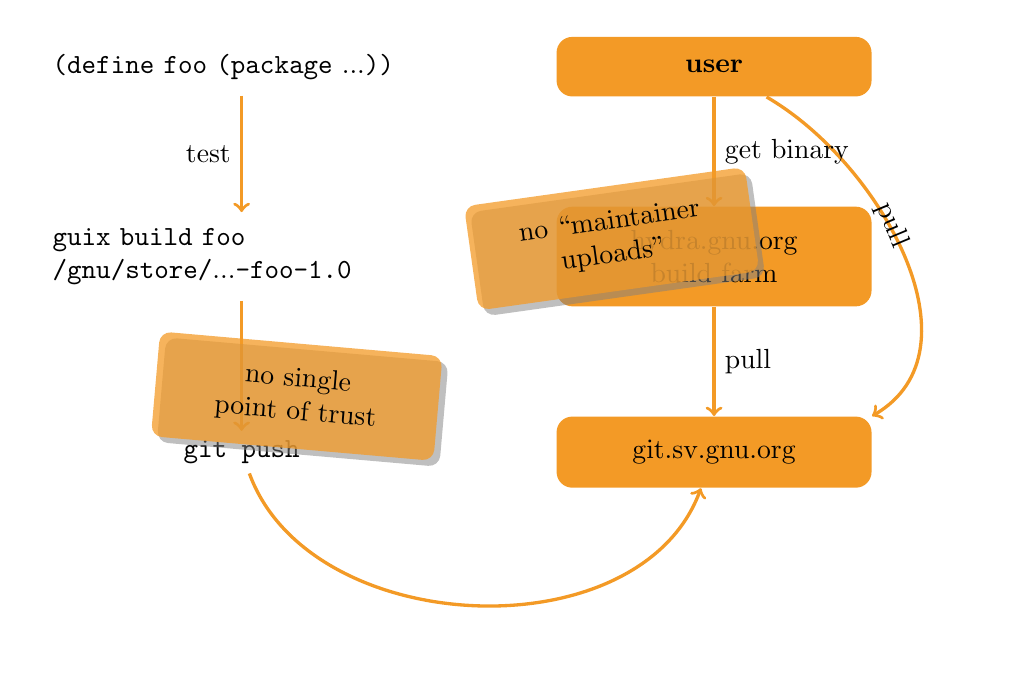
\begin{tikzpicture}[box/.style = {
                         rounded corners=2mm,
                         fill=white, text=black, text width=4.8cm,
                         inner sep=2mm
                      },
                      server/.style = {
                         text centered, rounded corners=2mm,
                         fill=guixorange1, text=black, text width=3.4cm,
                         inner sep=3mm
                      },
                      note/.style = {
                        rounded corners=4, text centered,
                        fill=guixorange1, text width=3cm,
                        inner sep=3mm, rotate=5, opacity=.75, text opacity=1,
                        drop shadow={opacity=0.5}
                      }]
    \matrix[row sep=1.4cm, column sep=1.4cm] {
      \node(def)[box]{\texttt{(define foo (package \textrm{...}))}};
      & \node(user)[server]{\textbf{user}};
      \\
      \node<2->(build)[box]{\texttt{guix build foo}
         \texttt{/gnu/store/\textrm{...}-foo-1.0}};
      & \node<4-5>(hydra)[server]{hydra.gnu.org build~farm};
      \\
      \node<3->(push){\texttt{git push}};
      & \node<3->(savannah)[server]{git.sv.gnu.org}; \\
      \\
    };

    \path[->, very thick, draw=guixorange1]<2->
      (def) edge node[left]{test} (build);
    \path[->, very thick, draw=guixorange1]<3->
      (build) edge (push);
    \path[->, very thick, draw=guixorange1]<3->
      (push) edge[->, in=-110, out=-70] (savannah);
    \path[->, very thick, draw=guixorange1]<4-5>
      (hydra) edge node[right]{pull} (savannah);
    \path[->, very thick, draw=guixorange1]<4-6>
      (user) edge[in=30,out=-30] node[left, sloped]{pull}
      (savannah.north east);
    \path[->, very thick, draw=guixorange1]<5>
      (user) edge node[right]{get binary} (hydra);

    \node<7>[overlay, fill=black, opacity=.8, 
             text height=8cm, text width=11cm,
             at=(current page.center)] {};

    \node<7>[note, rotate=3] at (2,1) {no ``maintainer uploads''};
    \node<7>[note, rotate=-10] at (-2,-1) {no single point of trust};
  \end{tikzpicture}
\end{frame}

%% \begin{frame}[plain]

%%   \begin{tikzpicture}[overlay]
%%     \node (hellobuilddeps) [at=(current page.center), inner sep=0] {%
%%       \includegraphics[width=\paperwidth]{images/hello-buildtime-deps}%
%%     };

%%     \node<2-> (bootbinlabel) at (6cm,2.5cm) {%
%%       \textbf{bootstrap} binaries%
%%     };
%%     \node<1> (hellobuilddepslabel) at (6cm,-4.5cm) {%
%%       build-time dependencies of GNU Hello%
%%     };
%%     \path[->]<1> (hellobuilddepslabel.north) edge [bend left, in=180] (hellobuilddeps.south);
%%     \path[->]<2> (bootbinlabel.south) edge [bend left, in=180] (hellobuilddeps.north);
%%     %% \path[->]<3> (hellobuilddepslabel.north)
%%     %%    edge [bend right, in=-90, out=-90, very thick]
%%     %%    node [below, sloped] {\large{can we close the loop?}}
%%     %%    (hellobuilddeps.north);
%%   \end{tikzpicture}
%% \end{frame}

\begin{frame}[plain]
  \LARGE{does this binary \alert{\textbf{correspond}}\\[3mm]
    to that source?}
\end{frame}

\begin{frame}[fragile]
  \frametitle{towards deterministic builds}

  \begin{semiverbatim}
\$ guix build guile
\uncover<2->{/gnu/store/\tikz[baseline]{\node[anchor=base](nixhash){\alert<2>{h2g4sc09h4...}};}-guile-2.0.9}

\uncover<3->{\$ \alert<3>{guix gc --references /gnu/store/...-guile-2.0.9}
/gnu/store/4jl83jgzaac...-glibc-2.17
/gnu/store/iplay43cg58...-libunistring-0.9.3
/gnu/store/47p47v92cj9...-libffi-3.0.9
/gnu/store/drkwck2j965...-gmp-5.0.5
...}
  \end{semiverbatim}

  \begin{tikzpicture}[overlay]
    \node<1>(labelnixhash) [fill=white, text=black] at (current page.center) {%
      \Large{\textbf{isolated build}: chroot, separate name spaces, etc.}
    };

    \node<2>(labelnixhash) [fill=white, text=black] at (4cm, 2cm) {%
      hash of \textbf{all} the dependencies};
    \path[->]<2>(labelnixhash.north) edge [bend left, in=180, out=-45] (nixhash.south);

    \draw<4> (-10pt, 105pt) [very thick, color=guixorange2, rounded corners=8pt]
      arc (10:-50:-50pt and 110pt);
    \node<4>[fill=white, text=black, text opacity=1, opacity=.7,
          rounded corners=2mm, inner sep=5mm]
      at (7, 2) {\textbf{(nearly) bit-identical for everyone}};
  \end{tikzpicture}

\end{frame}


\begin{frame}[plain]
  \begin{tikzpicture}[overlay]
    % http://www.heise.de/ct/artikel/NSA-GCHQ-The-HACIENDA-Program-for-Internet-Colonization-2292681.html?hg=1&hgi=8&hgf=false
    \node [at=(current page.center), inner sep=0mm]
    {\includegraphics[height=\paperheight]{images/sigint-rice}};

    \node<2>[rounded corners=4, text centered,
          fill=guixorange1, text width=10cm,
          inner sep=2mm, rotate=5, opacity=.75, text opacity=1,
          drop shadow={opacity=0.5}] at (current page.center) {
      \LARGE{\textbf{do not \alert{trust} a single\\ binary provider}}
    };
  \end{tikzpicture}
\end{frame}

\begin{frame}[plain]
  \vspace{1cm}
  % \hfill{\url{https://blog.torproject.org/blog/deterministic-builds-part-one-cyberwar-and-global-compromise}}
  \textrm{\Large{Deterministic Builds: Integrity\\
      through Decentralization}}

  \vspace{0.6cm}
  \hfill{\large{-- Mike Perry}}
\end{frame}


\begin{frame}[plain]
  \Huge{\alert{cool features} for\\[5mm]
    \textbf{GNU maintainers}}
\end{frame}

\begin{frame}[plain, fragile]
  \begin{semiverbatim}
\$ guix package -i gettext
\only<1>{looking for \alert{latest release of GNU gettext...}}\uncover<2>{note: using 0.18.3 but \alert{0.19.2 is available upstream}}
  \end{semiverbatim}
\end{frame}

\begin{frame}[plain, fragile]
  \begin{semiverbatim}
    \large{
\$ guix build emacs\uncover<2->{ \\
 --with-source=ftp://alpha.gnu.\textrm{...}/emacs-24.3.92.tar.xz
      }
    }
  \end{semiverbatim}

  \begin{tikzpicture}[overlay]
    \node<3>[rounded corners=4, text centered,
      fill=guixorange1, text width=7cm,
      inner sep=3mm, opacity=.5, text opacity=1,
      drop shadow={opacity=0.5}] at (current page.center) {
      \Large{\textbf{pre-release testing in a pristine environment}}
    };
  \end{tikzpicture}
\end{frame}

\begin{frame}[plain, fragile]
  \begin{tikzpicture}[overlay]
    \node [at=(current page.center), inner sep=0mm]
    {\includegraphics[width=\paperwidth]{images/daiki-libunistring-rc}};

    \node<2>[rounded corners=4, text centered,
      fill=guixorange1, text width=7cm,
      inner sep=3mm, rotate=5, opacity=.75, text opacity=1,
      drop shadow={opacity=0.5}] at (current page.center) {
      \Large{\textbf{send a package recipe!  :-)}}
    };
  \end{tikzpicture}
\end{frame}

\begin{frame}[plain, fragile]
  \begin{semiverbatim}
(use-modules (guix) (gnu))

(package (\alert{inherit}
          (car (find-packages-by-name "libunistring")))
  (version "0.9.4rc1")
  (source (origin
            (method url-fetch)
            (uri "http://\textrm{...}/libunistring-0.9.4-rc1.tar.gz")
            (sha256 (base32 "14pi90\textrm{...}")))))


\uncover<2->{$ guix build -e '(load "libunistring-rc.scm")'
The following derivations will be built:
   /gnu/store/\textrm{...}-libunistring-0.9.4rc1.drv
   /gnu/store/\textrm{...}-libunistring-0.9.4-rc1.tar.gz.drv
}
  \end{semiverbatim}

  \begin{tikzpicture}[overlay]
    \node<3>[rounded corners=4, text centered,
      fill=guixorange1, text width=10cm,
      inner sep=3mm, rotate=0, opacity=.75, text opacity=1,
      drop shadow={opacity=0.5}] at (current page.center) {
      \Large{\textbf{but does, say, Guile work with the RC?}}
    };
  \end{tikzpicture}
\end{frame}

\begin{frame}[plain, fragile]
  \begin{semiverbatim}
(use-modules (gnu packages guile) (guix)
             (srfi srfi-1))

(package (inherit guile-2.0)
  \alert{;; Replace the stable libunistring with the RC}
  \alert{;; in Guile's dependencies.}
  (inputs `(("libunistring"
               ,(primitive-load "libunistring-rc.scm"))
            ,@(alist-delete "libunistring"
                            (package-inputs guile-2.0)))))


\uncover<2->{\$ guix build -e '(load "guile-libunistring.scm")'
The following derivations will be built:
   /gnu/store/\textrm{...}-guile-2.0.11.drv
   /gnu/store/\textrm{...}-libunistring-0.9.4-rc1.tar.gz.drv
   /gnu/store/\textrm{...}-libunistring-0.9.4rc1.drv
}
  \end{semiverbatim}

  \begin{tikzpicture}[overlay]
    \node<3>[rounded corners=4, text centered,
      fill=guixorange1, text width=7cm,
      inner sep=3mm, opacity=.5, text opacity=1,
      drop shadow={opacity=0.5}] at (current page.center) {
      \Large{\textbf{reliable integration testing}}
    };
  \end{tikzpicture}
\end{frame}

\begin{frame}
  \frametitle{\huge{even better}}
  \framesubtitle{\uncover<2>{(left as an exercise to the audience)}}

  \Large{
    \begin{enumerate}
    \item \textbf{iterate} over the packages with \texttt{fold-packages}
    \item identify those \textbf{depending on libunistring}
    \item compute \textbf{package variants} that use the RC
    \item \textbf{build them}
    \end{enumerate}
  }
\end{frame}


%%%%%%%%%%%%%%%%%%%%%%%%%%%%%%%%%%%%%%%%%%%%%%%%%%%%%%%%%%%%%%%%%%%%%%%%%%%%%%%%
\begin{frame}[plain]
  \begin{centering}
    \Huge{\textbf{Hackable.}}
  \end{centering}
\end{frame}

\begin{frame}[plain]
  \frametitle{}
  
  \vspace{0.5cm}
  \textrm{\LARGE{%
      The truth is that Lisp is not the right language for
      any particular problem.  Rather, Lisp encourages one to attack a
      new problem by \alert{implementing new languages} tailored to that
      problem.  }}

  \vspace{1cm}
  \hfill{-- Abelson \& Sussman, 1987}
\end{frame}

\begin{frame}[fragile]
  \begin{semiverbatim}
(define hello
  (\alert{package}
   (name "hello")
   (version "2.8")
   (source (\alert{origin}
            (method url-fetch)
            (uri (string-append
                  "mirror://gnu/\textrm{...}/hello-" version
                  ".tar.gz"))
            (sha256 (base32 "0wqd\textrm{...}dz6"))))
   (\alert{build-system} gnu-build-system)
   (synopsis "Hello, GNU world: An example GNU package")
   (description "Produce a friendly greeting.")
   (home-page "http://www.gnu.org/software/hello/")
   (license gpl3+)))
  \end{semiverbatim}

  % \begin{tikzpicture}[overlay]
  %   \node[rounded corners=4, text centered,
  %         fill=guixorange1, text width=3cm,
  %         inner sep=3mm, rotate=-5, opacity=.75, text opacity=1,
  %         drop shadow={opacity=0.5},
  %         at=(current page.center)] {
  %           \textbf{\large{Emacs + Geiser demo!}}
  %         };
  % \end{tikzpicture}
\end{frame}

\begin{frame}[fragile]{}
  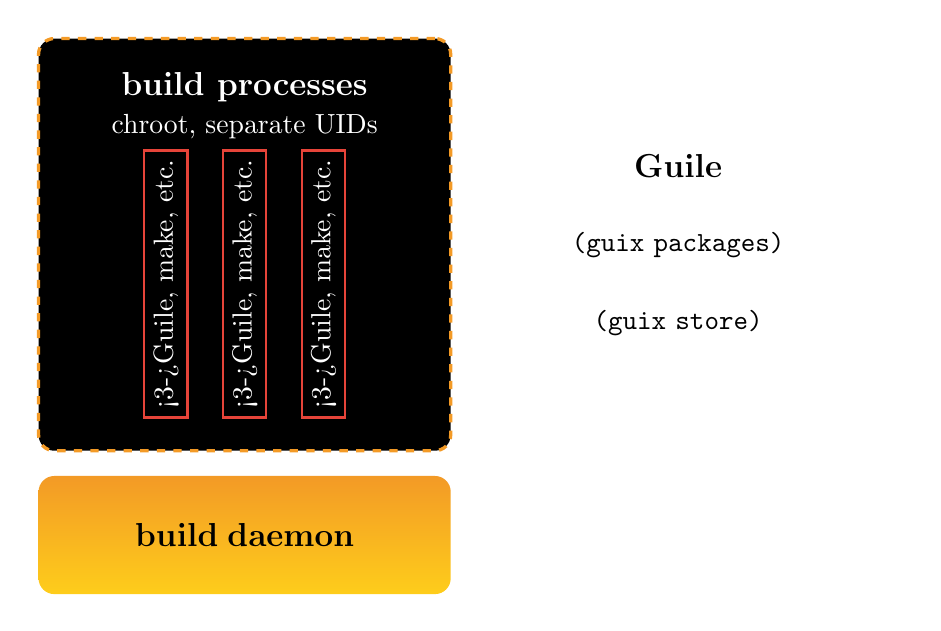
\begin{tikzpicture}[tools/.style = {
                        text width=35mm, minimum height=4cm,
                        text centered,
                        rounded corners=2mm,
                        fill=white, text=black
                      },
                      tool/.style = {
                        fill=white, text=black, text width=3cm,
                        text centered
                      },
                      daemon/.style = {
                        rectangle, text width=50mm, text centered,
                        rounded corners=2mm, minimum height=15mm,
                        top color=guixorange1,
                        bottom color=guixyellow,
                        text=black
                      },
                      builders/.style = {
                        draw=guixorange1, very thick, dashed,
                        fill=black, text=white, text width=5cm,
                        rounded corners=2mm,
                      },
                      builder/.style = {
                        draw=guixred2, thick, rectangle,
                        fill=black, text=white,
                        rotate=90
                      }]
    \matrix[row sep=3mm, column sep=1cm] {
      \node(builders)[builders, text height=5cm]{}
          node[fill=black, text=white] at (0, 2) {\large{\textbf{build processes}}}
          node[fill=black, text=white] at (0, 1.5) {chroot, separate UIDs}
          node[builder, onslide=<1-2>{black}] at (-1,-0.5) {\alert<3->{Guile}, make, etc.}
          node[builder, onslide=<1-2>{black}] at ( 0,-0.5) {\alert<3->{Guile}, make, etc.}
          node[builder, onslide=<1-2>{black}] at ( 1,-0.5) {\alert<3->{Guile}, make, etc.}; &
      \node[tools]{}
          node[fill=white, text=black] at (0, 1) {\large{\textbf{Guile}}}
          node[tool] at (0, 0) {\texttt{(guix packages)}}
          node(client)[tool] at (0, -1) {\texttt{(guix store)}};
      \\

      \node(daemon)[daemon]{\large{\textbf{build daemon}}}; &
      &
      \\
    };
  \end{tikzpicture}

  \begin{tikzpicture}[overlay]
    \path[very thick, draw=guixorange1]<2->
      (client.south) edge [out=-90, in=0, ->] node[below, sloped]{RPCs} (daemon.east);
    \path[->, very thick, draw=guixorange1]<3->
      (daemon) edge (builders);
  \end{tikzpicture}
\end{frame}


\begin{frame}[fragile]
  \begin{semiverbatim}
(\alert{use-modules} (guix) (gnu packages base))

\alert{,enter-store-monad}

(interned-file "README")
=> "/gnu/store/rwmzi9jlj77a7bq5kyiy2abdqznr3f02-README"

(gexp->derivation "list-files"
  \#~(symlink (string-append \#\$coreutils "/bin/ls")
             \#\$output))
=> \#<derivation "/gnu/store/xyz\textrm{...}-list-files\alert{.drv}" \textrm{...}>

(package->derivation hello)
=> \#<derivation "/gnu/store/xyz\textrm{...}-hello-2.8\alert{.drv} \textrm{...}>

(built-derivations (list drv))
\textsf{\alert{... daemon builds/downloads package on our behalf...}}
=> \#t

  \end{semiverbatim}

  \begin{tikzpicture}[overlay]
    \node[rounded corners=4, text centered,
          fill=guixorange1, text width=3cm,
          inner sep=3mm, rotate=-5, opacity=.75, text opacity=1,
          drop shadow={opacity=0.5},
          at=(current page.center)] {
            \textbf{\large{Emacs + Geiser demo!}}
          };
  \end{tikzpicture}
\end{frame}


% \begin{frame}[fragile]{build expressions}
%   \begin{semiverbatim}
% (let* ((store   \tikz[baseline]{\node[anchor=base](conn){(open-connection)};})
%        (builder '(\tikz[baseline]{\node[anchor=base](builder){begin};}
%                    (mkdir \%output)
%                    (call-with-output-file
%                        (string-append \%output "/test")
%                      (lambda (p)
%                        (display '(hello guix) p)))))
%        (drv (\tikz[baseline]{\node[anchor=base](drv){\alert{build-expression->derivation}};}
%                store "foo" "x86\_64-linux"
%                builder
%                '(("HOME" . "/nowhere")))))
%   (\tikz[baseline]{\node[anchor=base](build){\alert{build-derivations}};} store (list drv)))
%   \end{semiverbatim}

%   % \begin{textblock}{6}(3, 2)
%   %   \tikz{\node<2>[fill=white, text=black](labelconn){connect to
%   %       the build daemon};}
%   % \end{textblock}

%   \begin{textblock}{6}(8, 2)
%     \tikz{\node<2>[fill=white, text=black](labelbuilder){build script,
%         to be eval'd in chroot};}
%   \end{textblock}

%   \begin{textblock}{4}(1, 6)
%     \tikz{\node<3>[fill=white, text=black, text width=4cm](labeldrv){compute derivation
%         for this builder, system, and env.~vars};}
%   \end{textblock}

%   \begin{textblock}{5}(1, 7)
%     \tikz{\node<4>[fill=white, text=black, text
%       width=4cm](labelguile){implicitly adds Guile as an input};}
%   \end{textblock}

%   \begin{textblock}{6}(1, 9)
%     \tikz{\node<5>[fill=white, text=black](labelbuild){build it!};}
%   \end{textblock}

%   \begin{tikzpicture}[overlay]
%     % \path[->, fill=white, thick]<2>(labelconn) edge (conn);
%     \path[->, fill=white, thick]<2>(labelbuilder) edge (builder);
%     \path[->, fill=white, thick]<3>(labeldrv) edge (drv);
%     \path[->, fill=white, thick]<4>(labelguile) edge (drv);
%     \path[->, fill=white, thick]<5>(labelbuild) edge (build);
%   \end{tikzpicture}
% \end{frame}

\begin{frame}[fragile]{}
  \begin{semiverbatim}
(package (\tikz[baseline]{\node(inherit)[anchor=base]{\alert{inherit}};} hello)
  (version "2.7")
  (source
    (origin
      (method url-fetch)
      (uri "mirror://gnu/hello/hello-2.7.tar.gz")
      (sha256
        (base32 "7dqw3...")))))
  \end{semiverbatim}

  \begin{textblock}{6}(7, 2)
    \tikz \node(labelinherit)[fill=white, text=black, text width=5.5cm]
      {copy fields from \texttt{hello} except for \texttt{version} and
        \texttt{source}};
  \end{textblock}
  
  \begin{tikzpicture}[overlay]
    \path[->] (labelinherit) edge (inherit);
  \end{tikzpicture}
\end{frame}

\begin{frame}[fragile]{}
  \begin{semiverbatim}
(define (static-package p)
  ;; Return a statically-linked variant of P.
  (package (\alert{inherit} p)
    (arguments
     `(\#:configure-flags '("--disable-shared"
                            "LDFLAGS=-static")
       ,@(package-arguments p)))))
  \end{semiverbatim}
\end{frame}

% \begin{frame}[fragile]{builder side of \texttt{gnu-build-system}}
%   \vspace{-0.4cm}
%   \begin{semiverbatim}
% (\alert{define} \%standard-phases
%   `((configure . ,configure)
%     (build . ,build)
%     ;; \textrm{...}
%     ))

% (\alert{define*} (gnu-build #:key (phases \%standard-phases)
%                     #:allow-other-keys
%                     #:rest args)
%   ;; Run all the PHASES in order, passing them ARGS.
%   (every (match-lambda
%           ((name . proc)
%            (format #t "starting phase `~a'~\%" name)
%            (let ((result (apply proc args)))
%              (format #t "phase `~a' done~\%" name)
%              result)))
%          phases))
%   \end{semiverbatim}
% \end{frame}

% \begin{frame}[fragile]{inserting a build phase}
%   \begin{semiverbatim}
% (define howdy
%   (\alert{package} (inherit hello)
%     (arguments
%       '(#:phases
%         (\tikz[baseline]{\node(alistcons)[anchor=base]{alist-cons-after};}
%           'configure 'change-hello
%           (lambda* (#:key system #:allow-other-keys)
%             (\tikz[baseline]{\node(subst)[anchor=base]{\alert<4>{substitute*}};} "src/hello.c"
%               (("Hello, world!")
%                (string-append "Howdy! Running on "
%                               system "."))))
%           \tikz[baseline]{\node(phases)[anchor=base]{\%standard-phases};})))))
%   \end{semiverbatim}

%   \begin{tikzpicture}[overlay]
%     \draw<2> (40pt, 145pt) [very thick, color=guixorange2, rounded corners=8pt]
%       arc (20:-40:-50pt and 110pt);
%     \node<2>[fill=white, text=black, text opacity=1, opacity=.7,
%           rounded corners=2mm, inner sep=5mm]
%       at (7, 4) {\textbf{builder-side expression}};
%   \end{tikzpicture}

%   \begin{textblock}{5}(1, 9)
%     \tikz{\node<3>[fill=white, text=black](labelphases){configure, build, check, install};}
%   \end{textblock}

%   \begin{textblock}{5}(8, 5)
%     \tikz{\node<3>(labelalistcons)[fill=white, text=black]{add a phase
%         before \texttt{configure}};}
%   \end{textblock}

%   \begin{textblock}{5}(5, 5)
%     \tikz{\node<4>(labelsubst)[fill=white, text=black]{patch things up à
%         la \texttt{sed}};}
%   \end{textblock}

%   \begin{tikzpicture}[overlay]
%     \path[->, fill=white, thick]<3>(labelphases) edge (phases);
%     \path[->, fill=white, thick]<3>(labelalistcons) edge (alistcons);
%     \path[->, fill=white, thick]<4>(labelsubst) edge (subst);
%   \end{tikzpicture}
% \end{frame}

\begin{frame}[plain]
  \huge{\textbf{and now, the operating system}}
\end{frame}

\begin{frame}[plain, fragile]
  \begin{semiverbatim}
(define my-config
  (\alert{operating-system}
   (host-name "gnubox")
   (timezone "Europe/Paris")
   (locale "en\_US.UTF-8")
   (bootloader (grub-configuration (device "/dev/sdX")))\uncover<2->{
   (\alert{initrd} (cut base-initrd <>
                 #:extra-modules '("usb-storage.ko")))}
   (file-systems (cons (file-system
                         (mount-point "/") \textrm{...})
                       %base-file-systems))
   (users (list (user-account
                  (name "ludo") (group "users")
                  (comment "Hello, this is me!")
                  (home-directory "/home/ludo"))))
   (packages (cons* iotop jnettop %base-packages)))
  \end{semiverbatim}
\end{frame}

\begin{frame}[plain, fragile]
  \begin{semiverbatim}
\$ guix system build os-config.scm
/gnu/store/lq5kbp84kl9q9ncbk578wa7x5x0lrl3f-system

\$ guix system vm os-config
/gnu/store/yan79p9k83dwk5yd6jgmhpjh0nxalfn6-run-vm.sh

\# guix system init os-config /mnt
\textrm{...}

\# guix system reconfigure os-config
\textrm{...}
  \end{semiverbatim}

  \begin{tikzpicture}[overlay]
    \node[rounded corners=4, text centered,
          fill=guixorange1, text width=3cm,
          inner sep=3mm, rotate=-5, opacity=.75, text opacity=1,
          drop shadow={opacity=0.5}] at (9,3) {
            \textbf{\large{demo!}}
          };
  \end{tikzpicture}
\end{frame}

%% \begin{frame}[plain, fragile]
%%   \begin{semiverbatim}
%% \small{
%% (\alert{expression->initrd}
%%  #~(begin
%%      (mkdir "/proc")
%%      (mount "none" "/proc" "proc")

%%      ;; Load Linux kernel modules.
%%      (let ((slurp (lambda (module)
%%                     (call-with-input-file
%%                         (string-append "/modules/" module)
%%                       get-bytevector-all))))
%%        (for-each (compose load-linux-module slurp)
%%                  (list "md4.ko" "ecb.ko" "cifs.ko")))

%%      ;; Turn eth0 up.
%%      (let ((sock (socket AF_INET SOCK_STREAM 0)))
%%        (set-network-interface-flags sock "eth0" IFF_UP))

%%      ;; At last, the warm and friendly REPL.
%%      (start-repl)))
%% }
%%   \end{semiverbatim}

%%   \begin{tikzpicture}[overlay]
%%     \node[rounded corners=4, text centered,
%%           fill=guixorange1, text width=3cm,
%%           inner sep=3mm, rotate=-10, opacity=.75, text opacity=1,
%%           drop shadow={opacity=0.5}] at (9,8) {
%%             \textbf{\large{boot to Guile!}}
%%           };
%%   \end{tikzpicture}
%% \end{frame}

\begin{frame}[plain, fragile]
  \begin{semiverbatim}
# deco status dmd
Started: (term-tty1 term-tty2 nscd syslog)
Stopped: ()

# deco stop nscd
Service nscd has been stopped
  \end{semiverbatim}

  \begin{tikzpicture}[overlay]
    \node[rounded corners=4, text centered,
          fill=guixorange1, text width=3cm,
          inner sep=3mm, rotate=-10, opacity=.75, text opacity=1,
          drop shadow={opacity=0.5}] at (8,5) {
            \textbf{\large{PID 1 is GNU dmd!}}
          };
  \end{tikzpicture}
\end{frame}

\begin{frame}
  \frametitle{GNU dmd in a nutshell}

  \large{
  \begin{itemize}
    \item born in \alert{2003}, revived in 2013 :-)
    \item dependency-based service manager
    \item<2-> \texttt{dmd} is PID 1, \texttt{deco} is a client
    \item<3-> written in \alert{Guile} Scheme
    \item<3-> dynamic, extensible, etc.
  \end{itemize}}
\end{frame}


%%%%%%%%%%%%%%%%%%%%%%%%%%%%%%%%%%%%%%%%%%%%%%%%%%%%%%%%%%%%%%%%%%%%%%%%%%%%%%%%
\begin{frame}[plain, fragile]
  \begin{centering}
    \Huge{\textbf{extra coolness}}
  \end{centering}

  \begin{tikzpicture}[overlay]
    \node [at={(9,-2)}] {
      \includegraphics[width=0.4\paperwidth]{images/free-bonus}
    };
  \end{tikzpicture}
\end{frame}

\begin{frame}[fragile]
  \frametitle{GNU/Hurd port---the true GNU!}
  \framesubtitle{WIP by Manolis Ragkousis}

  \Large{
  \begin{itemize}
  \item step \#1: cross-compiling to GNU/Hurd
  \item<2-> packaged Mach, MiG, the Hurd, and...
  \item<2-> ... libc
  \item<3-> but! GNU libc \textbf{fails to build} on GNU/Hurd
  \item<4-> \large{(Debian's version does build...)}
  \end{itemize}
  }

  \begin{tikzpicture}[overlay]
    \node<5>[rounded corners=4, text centered,
      fill=guixorange1, text width=7cm,
      inner sep=3mm, rotate=5, opacity=.75, text opacity=1,
      drop shadow={opacity=0.5}] at (5, 2) {
      \Large{\textbf{help the Hurd \& libc regain harmony!}}
    };
  \end{tikzpicture}
\end{frame}

\begin{frame}[plain]
  \begin{tikzpicture}[remember picture, overlay]
    \node [at=(current page.center), inner sep=0pt]
          {\includegraphics[width=\paperwidth]{images/guix-web}};

    \node<1>[rounded corners=4, text centered,
      fill=guixyellow, text=black, text width=5cm,
      inner sep=3mm, rotate=-10, opacity=.75, text opacity=1,
      drop shadow={opacity=0.5}] at (8, 2) {
      \Huge{\textbf{world première!}}
    };

    \node<2> [text=black, text ragged, text width=10cm] at (8, 2) {
      \large{\textbf{WIP by David Thompson}}\\
      \texttt{https://gitorious.org/guix-web/guix-web}
    };
  \end{tikzpicture}
\end{frame}

\begin{frame}[plain]
  \begin{tikzpicture}[remember picture, overlay]
    \node<1> [at=(current page.center), inner sep=0pt]
          {\includegraphics[width=\paperwidth]{images/guix-el-list}};
    \node<2-> [at=(current page.center), inner sep=0pt]
          {\includegraphics[width=\paperwidth]{images/guix-el-package}};
  \end{tikzpicture}

  \begin{tikzpicture}[overlay]
    \node<1-2>[rounded corners=4, text centered,
      fill=guixyellow, text=black, text width=5cm,
      inner sep=3mm, rotate=-10, opacity=.75, text opacity=1,
      drop shadow={opacity=0.5}] at (8, 2) {
      \Huge{\textbf{guix.el!}}
    };

    \node<3> [text=white, text ragged, text width=7.5cm,
      fill=white, opacity=.3, text opacity=1,
      rounded corners=4, inner sep=3mm] at (7, 1.5) {
      \large{\textbf{WIP by Alex Kost}}\\
      \texttt{https://github.com/alezost/guix.el}\\(merged soon)
    };
  \end{tikzpicture}
\end{frame}

%% TODO: Add architecture diagrams

\begin{frame}[plain]
  \Large{$\Rightarrow$ plan working
    \textbf{as expected}}
  \\[1cm]
  \uncover<2->{\Huge{\textbf{embed DSLs!}}}
\end{frame}

%%%%%%%%%%%%%%%%%%%%%%%%%%%%%%%%%%%%%%%%%%%%%%%%%%%%%%%%%%%%%%%%%%%%%%%%%%%%%%%%
\begin{frame}[plain]
  \begin{centering}
    \Huge{\textbf{Lively!}}
  \end{centering}
\end{frame}

\begin{frame}{timeline}
  \begin{itemize}
    \item July 2012 --- GHM, Düsseldorf
    \item Nov. 2012 --- dubbed GNU
    \item{Jan. 2013 --- \alert{0.1}}
    \item{June 2013 --- European Lisp Symposium}
    \item{27 Sep. 2013 --- \alert{0.4}, with VM image}
    \item{Dec. 2013 --- \alert{0.5}, system config, mips64}
    \item{Apr. 2014 --- \alert{0.6}, signed binaries, \texttt{guix
        system}}
    \item<2>{July 2014 --- \alert{0.7}, \textbf{installable operating
        system!}}
  \end{itemize}
\end{frame}


\begin{frame}[plain]
  \frametitle{status}
  \begin{tikzpicture}[overlay]
    % http://en.wikipedia.org/wiki/File:Kibbles_How_Others_See_Me.jpg
    \node [at=(current page.center), inner sep=0mm]
    {\includegraphics[width=\paperwidth]{images/dog-food}};

    \node [text=white] at (current page.center) { \Huge{\textbf{status}} };
  \end{tikzpicture}
\end{frame}

\begin{frame}{status}
  \large{
  \begin{itemize}
    \item full-featured package manager
    \item 900 packages, 3 platforms
    \item \textbf{standalone distro!} (alpha)
    \item binaries built \& served at \url{http://hydra.gnu.org}
    \item tooling: auto-update, sync descriptions with GNU, etc.
    \item l10n: 7 languages!
  \end{itemize}}
\end{frame}

\begin{frame}[plain]
  \begin{tikzpicture}[overlay]
    % http://www.ohloh.net/p/gnuguix
    \node [at=(current page.center), inner sep=0mm]
    {\includegraphics[width=0.9\paperwidth]{images/ohloh-commits}};
  \end{tikzpicture}
\end{frame}

% \begin{frame}{status}
%   \begin{itemize}
%     \item{community!
%         \begin{itemize}
%           \item<2-> 4+ regular contributors
%         \end{itemize}}
%     \item<3-> active repo, active mailing list, IRC channel
%     \item<3-> \url{http://bugs.gnu.org/guix} + \texttt{guix-devel@gnu.org}
%   \end{itemize}
% \end{frame}

\begin{frame}[plain]

  \begin{tikzpicture}[remember picture, overlay]
    \node [at=(current page.center), inner sep=0pt]
      {\includegraphics[width=\paperwidth]{images/ohloh-summary}};
    % \fill (0,0) circle (2pt);
    % \fill (10,0) [fill=red] circle (2pt);
    % \fill (0,4) [fill=green] circle (2pt);
    % \fill (10,4) [fill=blue] circle (2pt);
    \path[very thick, draw=red] (3.9cm, -3.6cm)
      edge [bend left, in=-60, out=-60] (7.1cm,-3.3cm);
  \end{tikzpicture}
\end{frame}

\begin{frame}{thanks for the code, reports, ideas, and translations!}

  \begin{itemize}
    \item Eric Bavier, Taylan Ulrich Bayirli/Kammer, John Darrington,
      Eelco Dolstra~\& the Nix~crew, Andreas Enge, Alírio Eyng, Guy
      Grant, Raimon Grau, Nikita Karetnikov, Aljosha Papsch, Manolis
      Ragkousis, Cyril Roelandt, Alex Sassmannshausen, Cyrill Schenkel,
      Jason Self, Sree Harsha Totakura, David Thompson, Mark H. Weaver
    \item Lluís Batlle i Rossell, Marek Benc, Daniel
      Clark, Alexandru Cojocaru, Aleix Conchillo Flaqué, Rafael
      Ferreira, Christian Grothoff, Jeffrin Jose, Kete, Alex Kost,
      Matthew Lien, Niels Möller, Yutaka Niibe, Adam Pribyl, Benno
      Schulenberg, Alen Skondro, Matthias Wachs, Zerwas
    \item Pavel Fric, Mario Blättermann, Felipe Castro, Balázs Úr,
      Rafael Ferreira, Miroslav Nikolic, Tran Ngoc Quân
      % Мирослав Николић
      % Trần Ngọc Quân
  \end{itemize}
\end{frame}

\begin{frame}{the road to 1.0}
  \Large{
    \begin{enumerate}
    \setcounter{enumi}{-1}
    \item \textbf{official FSDG compliance}
    \item \textbf{OS features}: dm-crypt, LVM, etc.
    \item \textbf{more service definitions}
    \item<2-> improved \texttt{guix system reconfigure}
    \item<3-> \textbf{authenticated} \texttt{guix pull} (signed commits?)
    \item<4-> \textbf{user interfaces}: Emacs, web, curses(?)
    \item<5-> larger, more robust \textbf{build farm}...
    \item<5-> less dog food...
    \item<5-> more packages...
    \item<6-> \textit{your idea here}
    \end{enumerate}
  }

\end{frame}

\begin{frame}[plain]

  \vspace{0.7cm}
  \Large{
    \begin{itemize}
    \item \textbf{install the distribution}
    \item \textbf{use it}, report bugs, add packages
    \item help with the \textbf{infrastructure} + admin
    \item share your \textbf{ideas}!
    \end{itemize}
  }

  \begin{textblock}{5}(7,8)
    \tikz
    \node[overlay, rounded corners=4, text centered,
          minimum size=10mm, fill=guixorange1, text width=5cm,
          inner sep=3mm, rotate=-7, opacity=.75, text opacity=1,
          drop shadow={opacity=0.5}] at (3, 3) {
            \textbf{your help needed!}
          };
  \end{textblock}
\end{frame}

\begin{frame}{}

\vfill{
  \vspace{6.5cm}
  \hfill{\includegraphics[width=0.3\textwidth]{images/guix-logo-white}}\\[0.2cm]
  \texttt{ludo@gnu.org} \hfill{\alert{\url{http://gnu.org/software/guix/}}}
}

\end{frame}

\begin{frame}{credits}
  \small{
  \begin{itemize}
  \item GNU Guix logo, GFDL, \url{http://gnu.org/s/guix/graphics}
  \item NSA SIGDEV slide,
    \url{http://www.heise.de/ct/artikel/NSA-GCHQ-The-HACIENDA-Program-for-Internet-Colonization-2292681.html}
  \item dog food,
    \url{http://en.wikipedia.org/wiki/File:Kibbles_How_Others_See_Me.jpg}
  \item commit stats \& project summary,
    \url{http://www.ohloh.net/p/gnuguix}
  \end{itemize}
  }
\end{frame}

\begin{frame}{}

  \begin{textblock}{12}(2, 8)
    \tiny{
      Copyright \copyright{} 2010, 2012, 2013, 2014 Ludovic Courtès \texttt{ludo@gnu.org}.

      Copyright of other images included in this document is held by
      their respective owners.
      \\[3.0mm]
      This work is licensed under the \alert{Creative Commons
        Attribution-Share Alike 3.0} License.  To view a copy of this
      license, visit
      \url{http://creativecommons.org/licenses/by-sa/3.0/} or send a
      letter to Creative Commons, 171 Second Street, Suite 300, San
      Francisco, California, 94105, USA.
      \\[2.0mm]
      At your option, you may instead copy, distribute and/or modify
      this document under the terms of the \alert{GNU Free Documentation
        License, Version 1.3 or any later version} published by the Free
      Software Foundation; with no Invariant Sections, no Front-Cover
      Texts, and no Back-Cover Texts.  A copy of the license is
      available at \url{http://www.gnu.org/licenses/gfdl.html}.
      \\[2.0mm]
      % Give a link to the 'Transparent Copy', as per Section 3 of the GFDL.
      The source of this document is available from
      \url{http://git.sv.gnu.org/cgit/guix/maintenance.git}.
    }
  \end{textblock}
\end{frame}


\end{document}

% Local Variables:
% coding: utf-8
% comment-start: "%"
% comment-end: ""
% ispell-local-dictionary: "american"
% compile-command: "rubber --pdf guix-ghm-2014.tex"
% End:
